\documentclass{../../../oss-classkick}

\begin{document}
\genheader

\gentitle{C}{HARMONIC MOTION}

\genmultidirections

\gengravity

\raggedcolumns
\begin{multicols}{2}
  \begin{enumerate}[leftmargin=18pt]
  \item A mass oscillates on the end of a spring that obeys Hooke's law. Which
    of the following statements is true?
    \begin{enumerate}[nosep,leftmargin=18pt,label=(\Alph*)]
    \item The amplitude of oscillation is equal to the potential energy of the
      spring.
    \item The kinetic energy of the oscillating mass is constant.
    \item Maximum potential energy occurs when the mass reaches the
      equilibrium position.
    \item The potential energy of the spring at the amplitude is equal to the
      kinetic energy at the equilibrium position.
    \item The kinetic energy of the spring at the amplitude is equal to the
      potential energy at the equilibrium position.
    \end{enumerate}
    \vspace{.7in}
    
  \item A superball is dropped from a height of \SI{5.}{\metre} above a floor.
    The ball bounces off the floor in a perfectly elastic collision so that it
    rises to the same height with each bounce. The motion of the ball can be
    described as
    \begin{enumerate}[nosep,leftmargin=18pt,label=(\Alph*)]
    \item harmonic motion with a period of $2$ \si{\second}
    \item harmonic motion with a period of $1$ \si{\second}
    \item harmonic motion with a period of $1/2$ \si{\second}
    \item motion with a constant velocity
    \item motion with a constant momentum
    \end{enumerate}
    \vspace{.7in}
    
  \item An object oscillates in simple harmonic motion along the $x$-axis
    according to the equation $x = 6 \cos(4t)$. The period of oscillation of the
    object is
    \begin{enumerate}[nosep,leftmargin=18pt,label=(\Alph*)]
    \item $1/4$ s
    \item 4 s
    \item $\pi/4$ s
    \item $\pi/2$ s
    \item $4\pi$ s
    \end{enumerate}
    
  \item A mass $m$ oscillates on the end of a string of length $L$. The
    frequency of the pendulum is $f$. How would you increase the frequency of
    the pendulum to $2f$?
    \begin{center}
      \begin{tikzpicture}[scale=1.1]
        \fill [pattern=north east lines] (-2,4) rectangle (2,4.2);
        \draw[ultra thick] (-2,4)--(2,4);
        \draw[thick,
          decoration={aspect=.3,segment length=2mm, amplitude=2.5mm, coil},
          decorate] (-1,4)--(-1,3);
        \draw[thick,
          decoration={aspect=.3,segment length=2mm, amplitude=2.5mm, coil},
          decorate] (1,4)--(1,3);
        \draw[fill=gray!70](-1.5,3) rectangle(1.5,2);
      \end{tikzpicture}
    \end{center}
    \begin{enumerate}[nosep,leftmargin=18pt,label=(\Alph*)]
    \item Increase the length of the pendulum to $4L$
    \item Decrease the length of the pendulum to $L/4$
    \item Increase the length of the pendulum to $2L$
    \item Decrease the length of the pendulum to $L/2$
    \item Decrease the mass of the pendulum to $m/2$
    \end{enumerate}
    \vspace{.7in}
    
  \item A mass hangs from two parallel springs, each with the same spring
    constant $k$. Compared to the period $T$ of the same mass oscillating on
    one of the springs, the period of oscillation of the mass with both
    springs connected to it is
    \begin{enumerate}[nosep,leftmargin=18pt,label=(\Alph*)]
    \item $T/4$
    \item $T/\sqrt{2}$
    \item $T$ (unchanged)
    \item $2T$
    \item $4T$
    \end{enumerate}
    \columnbreak
    
  \item Which of the following is generally true for an object in simple
    harmonic motion on a spring of constant $k$?
    \begin{enumerate}[nosep,leftmargin=18pt,label=(\Alph*)]
    \item The greater the spring constant $k$, the greater the amplitude of the
      motion.
    \item The greater the spring constant $k$, the greater the period of the
      motion.
    \item The greater the spring constant $k$, the greater the frequency of the
      motion.
    \item The lower the spring constant $k$, the greater the frequency of the
      motion.
    \item The lower the spring constant $k$, the greater the kinetic energy of
      the motion.
    \end{enumerate}
    \vspace{.7in}
  \end{enumerate}
  
  \textbf{Questions \ref{first}--\ref{last}}: A harmonic oscillator follows the
  equation $\displaystyle\frac{d^2x}{dt^2}=-4x$. The spring constant $k$ is
  \SI{4}{\newton\per\metre}.
  \begin{enumerate}[leftmargin=18pt,resume]
  \item The angular frequency $\omega$ of the harmonic motion is
    \begin{enumerate}[nosep,leftmargin=18pt,label=(\Alph*)]
    \item zero
    \item\SI{2}{rad\per\second}
    \item\SI{4}{rad\per\second}
    \item\SI{8}{rad\per\second}
    \item\SI{16}{rad\per\second}
    \end{enumerate}
    \label{first}

  \item The mass $m$ oscillating on the spring is
    \begin{enumerate}[nosep,leftmargin=18pt,label=(\Alph*)]
    \item\SI{1}{\kilo\gram}
    \item\SI{2}{\kilo\gram}
    \item\SI{4}{\kilo\gram}
    \item\SI{8}{\kilo\gram}
    \item\SI{16}{\kilo\gram}
    \end{enumerate}
    
  \item The period $T$ of oscillation is
    \begin{enumerate}[nosep,leftmargin=18pt,label=(\Alph*)]
    \item zero
    \item $\pi/4$\si{\second}
    \item $\pi/2$\si{\second}
    \item $\pi$  \si{\second}
    \item $2\pi$ \si{\second}
    \end{enumerate}
    \label{last}
    
  \item A pendulum of length $L$ has a period of \SI{2}{\second} on Earth. A
    planetary explorer takes the same pendulum of length $L$ to another planet
    where its period is \SI{1}{\second}. The gravitational acceleration on the
    surface of this planet is most nearly
%    \begin{center}
%      \begin{tikzpicture}
%        \fill [pattern=north east lines] (-5,0)--(0,0)--(0,2)--(.2,2)--
%        (.2,-.2)--(-5,-.2)--cycle;
%        \draw[ultra thick] (-5,0)--(0,0)--(0,2);
%        \draw[decoration={aspect=.3,segment length=2mm, amplitude=2.5mm, coil},
%          decorate] (0,.5)--(-1,.5);
%        \draw[fill=gray!70](-2,0) rectangle(-1,1) node[above]{\SI{1}{\kg}};
%        \draw[fill=gray!70](-4.5,0) rectangle(-3.5,1) node[above]{\SI{1}{\kg}};
%        \draw[ultra thick,->](-4,.5)--(-2.8,.5) node[pos=1,right]{$v$};
%        \draw[very thick,dashed](-.5,-.5)--(-.5,1.5);
%      \end{tikzpicture}
%    \end{center}
    \begin{enumerate}[nosep,leftmargin=18pt,label=(\Alph*)]
    \item $8g$
    \item $4g$
    \item $2g$
    \item $g/2$
    \item $g/4$
    \end{enumerate}
  \end{enumerate}
\end{multicols}
\newpage

\genfreetitle{C}{SIMPLE HARMONIC MOTION}{6}

\genfreedirections

%\item A mass $m$ oscillates on an ideal spring of spring constant $k$ on a
%  frictionless horizontal surface. The mass is pulled aside to a distance $A$
%  from its equilibrium position, and released.
%  \begin{center}
%    \begin{tikzpicture}
%      \fill [pattern=north east lines] (5,0)--(0,0)--(0,2)--(-0.2,2)
%      --(-0.2,-0.2)--(5,-0.2)--cycle;
%      \draw[ultra thick] (5,0)--(0,0)--(0,2)--(-0.5,2);
%      \draw[decoration={aspect=0.3,segment length=2mm, amplitude=2.5mm, coil},
%        decorate] (0,0.5)--(1.5,0.5);
%      \draw[fill=gray!70](1.5,0) rectangle(2.5,1);
%      \draw[thick](2.5,0)--(2.5,-0.3) node[pos=1,below]{O};
%      \draw[thick](4,0)--(4,-0.3) node[pos=1,below]{A};
%    \end{tikzpicture}
%  \end{center} 
%  \begin{enumerate}[noitemsep]  
%  \item In terms of the given quantities, at what distance from the equilibrium
%    position is the potential energy of the mass equal to its kinetic energy?
%  \item In terms of the given quantities, what is the acceleration of the mass
%    when it is at the amplitude $A$?
%  \end{enumerate}
%%  \vspace{3in}
%  \newpage
%  
%\item A mass oscillates in simple harmonic motion as shown by the position $x$
%  vs. time $t$ graph below.
%  \begin{center}
%    \pic{.45}{oscillate.png}
%  \end{center}
%  \begin{enumerate}[noitemsep]  
%  \item What is the frequency of oscillation?
%  \item Write the equation that represents the speed of the mass as a function
%    of time.
%  \end{enumerate}
%  \newpage

% QUESTION TAKEN FROM 2010 AP PHYSICS C FREE-RESPONSE QUESTION MECH 3
\cpic{.3}{skier}
\begin{enumerate}
\item A skier of mass $m$ will be pulled up a hill by a rope, as shown above.
  The magnitude of the acceleration of the skier as a function of time $t$ can
  be modeled by the equations
  \begin{align*}
    a &=a_\text{max}\sin\left(\frac{\pi t}{T}\right)  &(0<t<T)&\\
    &=0 & (t\geq T)&
  \end{align*}
  where $a_\text{max}$ and $T$ are constants. The hill is inclined at an angle
  $\theta$ above the horizontal, and friction between the skis and the snow is
  negligible. Express your answers in terms of given quantities and fundamental
  constants.
  \begin{enumerate}
  \item  Derive an expression for the velocity of the skier as a function of
    time during the acceleration. Assume the skier starts from rest.
  \item Derive an expression for the work done by the net force on the skier
    from rest until terminal speed is reached.
  \item Determine the magnitude of the force exerted by the rope on the skier
    at terminal speed.
  \item Derive an expression for the total impulse imparted to the skier during
    the acceleration.
  \item Suppose that the magnitude of the acceleration is instead modeled as
    $a=a_\text{max}e^{-\pi t/2T}$ for all $t > 0$, where $a_\text{max}$ and $T$
    are the same as in the original model. On the axes below, sketch the graphs
    of the force exerted by the rope on the skier for the two models, from
    $t=0$ to a time $t>T$. Label the original model $F_1$ and the new model
    $F_2$.
    \begin{center}
      \begin{tikzpicture}[scale=.85]
        \draw[->,thick](0,0)--(10,0)node[pos=1,right]{$t$};
        \draw[->,thick](0,0)--(0,6) node[pos=1,above]{$F$};
        \draw[thick](-.2,1.5)--(.2,1.5)node[pos=0,left]{$mg\sin\theta$};
        \draw[thick](5.5,-.2)--(5.5,.2)node[pos=0,below]{$T$};
      \end{tikzpicture}
    \end{center}
  \end{enumerate}
  \newpage
  
\item In heavy seas, the bow of a battle ship undergoes a simple harmonic
  vertical pitching motion with a period of \SI{8.}{\second} and an amplitude
  of \SI{2.}{\metre}.
  \begin{enumerate}
  \item What is the maximum vertical velocity of the battle ship's bow?
  \item What is its maximum acceleration?
  \item An \SI{80}{\kilo\gram} sailor is standing on the scale in the bunk room
    in the bow. What are the maximum and minimum reading on the scale in
    newtons?
  \end{enumerate}
  \newpage
  
\item Show that for the situations in the figures below, the object of mass
  $m$ oscillates with a frequency of
  $\displaystyle f=\frac1{2\pi}\sqrt{\frac{k_\text{eff}}m}$ where $k_\text{eff}$
  is given by (a) $k_\text{eff}=k_1+k_2$ and (b)
  $\displaystyle\frac1{k_\text{eff}}=\frac1{k_1}+\frac1{k_2}$. Hint:
  find the net force on the mass and write $F=-k_\text{eff}x$. Note that in
  (b), the springs stretch by different amounts, the sum of which is $x$.
  
  (a)\hspace{5pt}
  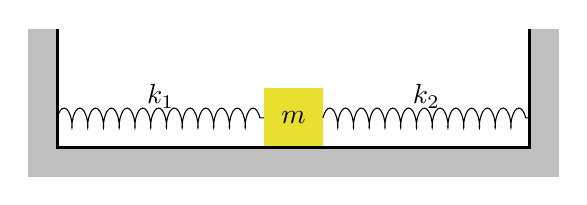
\begin{tikzpicture}[scale=.5]
    \fill[gray!50](0,0) rectangle(12,-.75);
    \fill[gray!50](-.75,-.75) rectangle(0,3);
    \fill[gray!50](12,-.75) rectangle(12.75,3);
    \fill[yellow!80!gray](5.25,0) rectangle(6.75,1.5) node[midway,black]{$m$};
    \draw[decoration={aspect=0.3,segment length=2mm, amplitude=1.25mm, coil},
      decorate] (0,.75)--(5.25,.75) node[midway,above]{$k_1$};
    \draw[decoration={aspect=0.3,segment length=2mm, amplitude=1.25mm, coil},
      decorate] (6.75,.75)--(12,.75) node[midway,above]{$k_2$};
    \draw[very thick](0,3)--(0,0)--(12,0)--(12,3);
  \end{tikzpicture}

  (b)\hspace{5pt}
  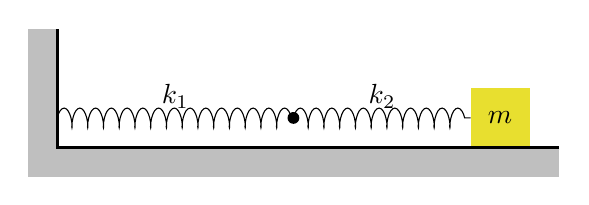
\begin{tikzpicture}[scale=.5]
    \fill[gray!50](0,0) rectangle(12.75,-.75);
    \fill[gray!50](-.75,-.75) rectangle(0,3);
    \fill[yellow!80!gray](10.5,0) rectangle(12,1.5) node[midway,black]{$m$};
    \draw[decoration={aspect=0.3,segment length=2mm, amplitude=1.25mm, coil},
      decorate] (0,.75)--(6,.75) node[midway,above]{$k_1$};
    \draw[decoration={aspect=0.3,segment length=2mm, amplitude=1.25mm, coil},
      decorate] (6,.75)--(10.5,.75) node[midway,above]{$k_2$};
    \fill[black](6,.75) circle(.15);
    \draw[very thick](0,3)--(0,0)--(12.75,0);
  \end{tikzpicture}
  \newpage
  
\item A simple pendulum of length $L$ is released from rest from an angle of
  $\theta_0$.
  \begin{enumerate}
  \item Assuming the motion of the pendulum to be simple harmonic motion, find
    its speed as it passes through $\theta=0$.
  \item Using the conservation of energy, find this speed exactly.
  \item Show that your results for (a) and (b) are the same when $\theta_0$ is
    small.
  \item Find the difference in your results for $\theta_0=\SI{.20}{rad}$ and
    $L=\SI1\metre$.
  \end{enumerate}
  \newpage

  \cpic{.35}{torsional}
\item The torsion pendulum shown above consists of a disk of rotational inertia
  $I$ suspended by a flexible rod attached to a rigid support. When the disk is
  twisted through a small angle $\theta$, the twisted rod exerts a restoring
  torque $t$ that is proportional to the angular displacement:
  $t=-\beta\theta$, where $\beta$ is a constant. The motion of a torsion
  pendulum is analogous to the motion of a mass oscillating on a spring.
  \begin{enumerate}
  \item In terms of the quantities given above, write but do NOT solve the
    differential equation that could be used to determine the angular
    displacement $\theta$ of the torsion pendulum as a function of time $t$.
  \item Using the analogy to a mass oscillating on a spring, determine the
    period of the torsion pendulum in terms of the given quantities and
    fundamental constants, as appropriate.
  \end{enumerate}
  To determine the torsion constant $\beta$ of the rod, disks of different,
  known values of rotational inertia are attached to the rod, and the data
  below are obtained from the resulting oscillations.
  \begin{center}
    \begin{tabular}{|c|c|c|c|}
      \hline
      Rotational Inertia $I$ of Disk (\si{\kilo\gram\metre\squared}) &
      Average Time for Ten Oscillations (s) &
      Period $T$ (s) & $T^2$ (\si{\second\squared}) \\\hline
      0.025 & 22.4 & 2.24 & 5.0  \\\hline
      0.036 & 26.8 & 2.68 & 7.2  \\\hline
      0.049 & 29.5 & 2.95 & 8.7  \\\hline
      0.064 & 33.3 & 3.33 & 11.1 \\\hline
      0.081 & 35.9 & 3.59 & 12.9 \\\hline
    \end{tabular}
  \end{center}
  \newpage
  
  \begin{enumerate}[resume]
  \item On the graph below, plot the data points. Draw a straight line that
    best represents the data.
    \cpic{.9}{graph-paper}
 
  \item Determine the equation for your line.
 
  \item Calculate the torsion constant $\beta$ of the rod from your line.
 
  \item What is the physical significance of the intercept of your line with
    the vertical axis?
  \end{enumerate}
\end{enumerate}
\end{document}
